\chapter{Deep Q-Learning}

Reinforcement Learning (RL) is an interesting technique for the design of a longitudinal controller and a lateral controller because it enables us to abstract from the complexity of car physics and dynamics that have an important computing cost. With algorithms such as Q-Learning, one can learn by choosing the actions and observing their results directly in the environment. Put into an ACC context, it is possible to learn an acting policy in a simulated highway system by taking actions on the cars' brakes and throttle, and observing the results. The policy obtained can be used as a longitudinal controller to safely follow a preceding vehicle. Similarly to an Lane Control, a lateral controller can be trained.

\section{General Architecture}

Our system follows the basic RL structure. The agent performs an action $A_t$ given state $S_t$ under policy $\pi$. The agent receives the state as feedback from the environment and gets the reward $r_t$ for the action taken. The state feedback that the agent takes from sensors consists of the velocities of the neighboring vehicles $v_{veh}[i] (i = 1, 2, ..., N)$ and the relative positions of the neighboring vehicles to the ego vehicle $dist_{veh}[i] (i = 1, 2, ..., N)$. Possible actions that agent can choose are among 4 levels of accelerations, 4 levels of decelerations and keeping the current speed. The goal of our proposed Deep Q-Learning System is to maximize the accumulated reward or ``value function'' \cite{Mnih2015AtariNature} that will be received in the future within an episode. Using the simulations, the agent learns from interaction with environment episode-by-episode. One episode starts when the vehicle and road state information are detected. The vehicle drives on a standard circular track. If the distance between the ego vehicle and the front vehicle or the behind vehicle is less than the safety distance $dist_{safe}$, it is considered as a collision event. The episode ends if at least one of the following events occurs

\begin{itemize}

\item \textbf{Collision} The ego vehicle detects the distance with the vehicle in front within $dist_{safe}$.

\item \textbf{Time Out} The maximal number of time steps are reached.

\item \textbf{Bump} The ego vehicle is turned over for some reason.

\item \textbf{Off Lane} The ego vehicle is out of lanes.

\end{itemize}

The ego vehicle continuously detects the space information in 6 areas around itself as shown in Fig \ref{fig:highway} and the maximal detecting range is 80 meters in front and behind. The variable $s_i (i = 0,1,...,5)$ represents the detected vehicle distance or obstacle distance along the path with the ego vehicle. If none is detected in the range of 80 meters, 80 would be put in the variable. For example, Vehicle 0 is located in the left lane of the ego vehicle and is behind it. Vehicle 0 is defined in Area 0. When there are multiple vehicles in the same area, only the closest is considered. Later we can use the information to check the state of the left lane or the right lane. A function is provided to compute if the lane change is safe or not.

\begin{figure}[h]
\centering
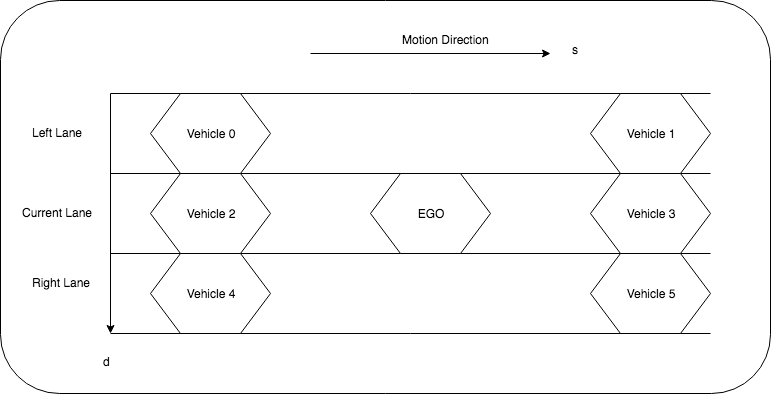
\includegraphics[width=0.8\textwidth]{figs/ch4/Highway-Display}
\caption{A general highway case display.}
\label{fig:highway}
\end{figure}

Once one episode ends, the next episode starts with the state of environment and the value function reset.

The general architecture is as shown in Fig. \ref{fig:diagram}.

\begin{figure}[h]
\centering
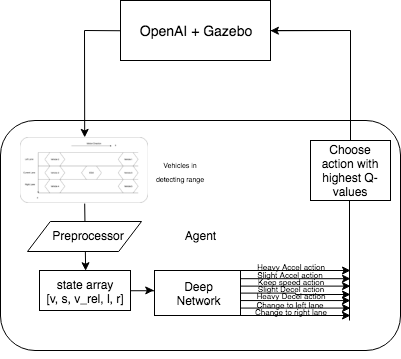
\includegraphics[width=0.8\textwidth]{figs/ch4/diagram}
\caption{A general architecture of training.}
\label{fig:diagram}
\end{figure}

OpenAI and Gazebo are providing online environment state information including the vehicle's state information. With the global path or the map given, we construct an array indicating the poses and velocities of the vehicles those are nearby the ego vehicle.

The preprocessor is to simplify and separate the in lane information for ACC and neighboring lane information for LC. Finally the state array to be fed into the Deep Network is a small and normalized array. The first three items ``v", ``s" and ``$v_{rel}$" are representing the speed of the ego vehicle $v_{ego}$, the distance between the ego vehicle and the preceding vehicle $s_{pre} - s_{ego}$ and the relative speed between the two, $v_{rel} = v_{pre} - v_{ego}$. The three are key variables for adaptive cruise control. The remaining two, $l$ and $r$, indicate the availabilities of the left lane and the right lane. The two are binary variables with ``True" representing that the lane is safe to reach. We define that only when there no vehicle detected within some range to the ego vehicle the target lane is thought to be available. Here we set 30 meters as the range limit. With this setting, we don't need to consider Adaptive Cruise Control problems when changing lane. After it changes to a new lane, the first three variables will also update to the state in the new lane and it will have enough time to adjust its speed with ACC.

The Deep Network will be trained to output Q-values for different classes of activities. The action with highest Q-value will be fed into OpenAI / Gazebo to generate the next state.

\section{Reinforcement Learning for Longitudinal Motion}

To apply this RL framework, we first had to model the problem by defining the states, actions, goals and rewards. Our first approach was to use variables such as the position of a leading car, their velocities and accelerations, etc. Clearly, this state definition put us up against the curse of dimensionality, and it became impossible to have a discrete state space precise enough to learn a valuable policy. We modified our state definition by consolidating numerous state variables. This allowed us to use a smaller discretization and to reach a better precision with only two variables. Since driving can be seen as a sequential decision problem, there is no problem in modeling it using a MDP and discrete state variables. For now, our discrete state space was built around a state definition containing variables as we defined our states by the relative distance and velocity between two vehicles.

This relative movement between vehicles is needed to take an informed decision on the action to take at the next time step. Those actions were taken directly on the brakes or throttle (only one action per time step is chosen), closely simulating human interaction. The actions were discretized, according to a percentage of pressure on the pedal, from accelerating, keeping to decelerating.

The goal is to maintain a high speed on highway and to slow down when detecting a slow vehicle ahead. To reach the goal, we set the rewards accordingly, with a positive reward proportional to the velocity (for a given time step it is the distance moved along the path). We also set negative rewards when wandering too close  with the preceding vehicle. The behavior the agent is supposed to learn is to maintain high speed and safe as long as possible.

Those elements were put together in a RL framework, and the policy obtained, learned in a simulated environment, formed the core of our longitudinal controller. The environment, a simulated highway system built in previous work, featured complex vehicle physics and dynamics as close as possible to reality. Since the simulation environment was using continuous time, we had to define the time interval at which action decisions would be taken. The action chosen at the specified time frame would be taken for the whole frame. To observe an accurate behavior of the vehicle, we had to set the time step between each action decision to a small value (50 milliseconds). But in such conditions, the observation of real vehicle acceleration needed many consecutive acceleration actions, a behavior that could not be learned in a decent time with normal state space exploration. 

\begin{figure}[h]
\centering
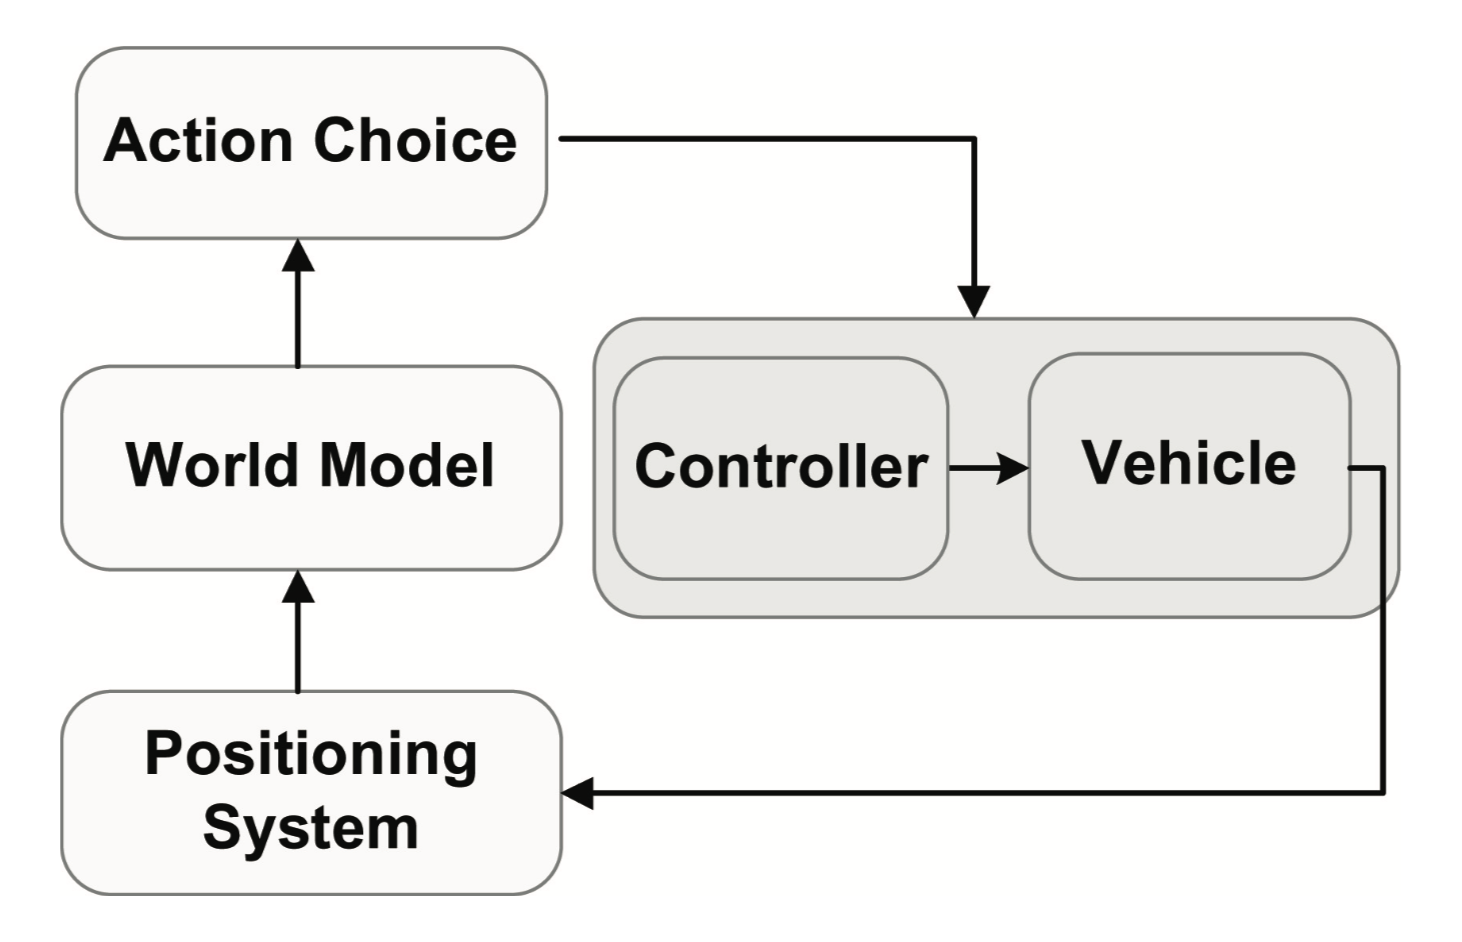
\includegraphics[width=0.8\textwidth]{figs/ch4/acc-drl}
\caption{Reinforcement applied on ACC system.}
\label{fig:acc-rl}
\end{figure}

Put into context, Fig. \ref{fig:acc-rl} shows that using RL simplifies the design of a longitudinal controller. The closed-loop controller takes as inputs the vehicle's state as described earlier, and selects the appropriate action according to the policy that was learned. Such a technique is obviously simpler than the complex mathematical analysis needed to predict precise car physics and dynamics for acting, as our controller basically hides in a black box vehicle physics and dynamics. It is possible for the agent to learn the optimal behavior by taking driving actions and observing their results on the time distance and its difference between two time steps. In the next section, we will show results obtained by using this policy for longitudinal vehicle control. As drivers spend a great amount of their time in heavy traffic, such systems could reduce the risk of rear-end collisions and protect the drivers mentally by relieving them from stressful driving.

\section{Reinforcement Learning for Lateral Motion}

Lateral motion control without longitudinal motion control hardly exists. Besides parking another good example of low speed combined longitudinal and lateral control is the traffic jam assist system. At speeds between zero and 40 or 60 km/h (depending on OEMs), the traffic jam assist system keeps pace with the traffic flow and helps to steer the car within certain constraints. It also accelerates and brakes autonomously. The system is based on the functionality of the adaptive cruise control with stop \& go, extended by adding the lateral control of steering and lane guidance. The function is based on the built-in radar sensors, a wide-angle video camera and the ultrasonic sensors of the parking system.

In this section, we describe the design of the Lane Control layer and, more precisely, the design of the policy to select the most efficient and safest lane for each vehicle according to their current state and action. Lane changes are stressful maneuvers for drivers, particularly during high-speed traffic flows. As designed in the last Chapter, the Lane Control system is using a Finite State Machine (FSM) and hence RL is only responsible for choosing the optimal behavior or next Finite State. The action space consists of three actions, Change to Left, Keep Lane and Change to Right. To make such kind of decision, the agent needs to be aware of the nearby vehicle's position and state in both its current lane and nearby lane. We maintain an array combining a 6-dimensional relative position array which captures space information in 6 nearby locations as shown in Fig. \ref{fig:highway} for the Lateral Control agent. With the array, we can easily check if the neighboring lane is available to reach.

\section{Q Learning}

Q-learning is one of the popular RL methods which searches for the optimal policy in an iterative fashion. Basically, the Q-value function $q_{\pi} (s, a)$ is defined as

\begin{equation}
q_\pi(s,a) = \mathbb{E}_\pi \left[ \sum _{k=0}^{\infty} \gamma ^k r_{t+k+1} | S_t = s, A_t = a \right]
\end{equation}

For the given state $s$ and action $a$, where $r_t$ is the reward received at the time step $t$. The Q-value function is the expected sum of the future rewards which indicates how good the action $a$ is given the state $s$ under the policy of the agent $\pi$. The contribution to the Q-value function decays exponentially with the discounting factor $\gamma$ for the rewards with far-off future. For the given Q-value function, the greedy policy is obtained as

\begin{equation} \label{eq:402}
\pi(s) = arg \max_a q_{\pi} (s, a) 
\end{equation}

One can show that for the policy in Eq. \ref{eq:402}, the following Bellman equation should hold,

\begin{equation}
q_\pi(s,a) = \mathbb{E}_\pi [r_{t+1} + \gamma \max_a q_\pi(S_{t+1},a) | S_t = s, A_t = a]
\end{equation}

In practice, since it is hard to obtain the exact value of $q_{\pi}(s, a)$ satisfying the Bellman equation, the Q-learning method uses the following update rule for the given one step backups $S_t$, $A_t$, $r_{t+1}$, $S_{t+1}$;

\begin{equation}
q_\pi(S_t,A_t) \gets q_\pi(S_t,A_t) + \alpha \left[r_{t+1} + \gamma \max_a q_\pi(S_{t+1},a) - q_\pi(S_t,A_t)\right]
\end{equation}

However, when the state space is continuous, it is impossible to find the optimal value of the state-action pair $q_{\pi} (s, a)$ for all possible states. To deal with this problem, the DQN method was proposed, which approximates the state-action value function q(s, a) using the DNN, i.e., $q(s, a) = q_\theta(s, a)$ where $\theta$ is the parameter of the DNN. The parameter $\theta$ of the DNN is then optimized to minimize the squared value of the temporal difference error $\delta_t$

\begin{equation} \label{eq:delta-1}
\delta_t = r_{t+1} + \gamma \max_{a^ \prime} q_\theta(S_{t+1},a^ \prime) - q_\theta(S_t,A_t)
\end{equation}

For better convergence of the DQN, instead of estimating both $q(S_t,A_t)$ and $q(S_{t+1},a^ \prime)$ in  Eq. \ref{eq:delta-1}, we approximate $q(St,At)$ and $q(S_{t+1},a^ \prime)$ using the Q-network and the target network parameterized by $\theta$ and $\theta^{\prime}$, respectively. The update of the target network parameter $\theta^{\prime}$, is done by cloning Q-network parameter $\theta$, periodically. Thus, Eq. \ref{eq:delta-1} becomes

\begin{equation}
\delta_t = r_{t+1} + \gamma \max_{a^ \prime} q_{\theta^{\prime}}(S_{t+1},a^ \prime) - q_\theta(S_t,A_t)
\end{equation}

To speed up convergence further, replay memory is adopted to store a bunch of one step backups and use a part of them chosen randomly from the memory by batch size. The backups in the batch is used to calculate the loss function $L$ which is given by

\begin{equation}
L = \sum_{t\in B_{replay}}\delta_t^2
\end{equation}

where $B_{replay}$ is the backups in the batch selected from replay memory. Note that the optimization of parameter $\theta$ for minimizing the loss $L$ is done through the stochastic gradient descent method.

One of the most basic and popular methods to estimate action-value functions is the \emph{Q-learning} algorithm. It is model-free online off-policy algorithm, whose main strength is that it is able to compare the expected utility of the available actions without requiring a model of the environment. Q-learning works by learning an action-value function that gives the expected utility of taking a given action in a given state and following a fixed policy thereafter.

A value function estimates what is good for an agent over the long run. It estimates the expected outcome from any given state, by summarizing the total amount of reward that an agent can expect to accumulate into a single number. Value functions are defined for particular policies.

The \emph{state value function} (or V-function), is the expected return when starting in state $s$ and following policy $\pi$ thereafter~\citep{Sutton1998RL},
%
\begin{equation}
V^\pi(s) = \mathbb{E}_\pi \left[R_t | s_t = s \right]
\end{equation}

The \emph{action value function} (or Q-function), is the expected return after selecting action $a$ in state $s$ and then following policy $\pi$,
%
\begin{equation}
q^\pi(s,a) = \mathbb{E}_\pi \left[ R_t | s_t = s, a_t = a \right]
\end{equation}

The \emph{optimal value function} is the unique value function that maximizes the value of every state, or state-action pair,
%
\begin{eqnarray}
Q^*(s,a) & = & \max\limits_\pi Q^\pi(s,a), \forall s \in \mathcal{S}, a \in \mathcal{A}
\end{eqnarray}

An \emph{optimal policy} $\pi^*(s,a)$ is a policy that maximizes the action value function from every state in the MDP,
%
\begin{equation}
    \pi^*(s,a) = \argmax_\pi Q^\pi(s, a)
\end{equation}

The update rule uses action-values and a built-in max-operator over the action-values of the next state in order to update $Q(s_t, a_t)$ as follows,

\begin{equation}
Q(s_t,a_t) \gets Q(s_t,a_t) + \alpha \left[r_{t+1} + \gamma \max_a Q(s_{t+1},a) - Q(s_t,a_t)\right]
\end{equation}

The agent makes a step in the environment from state $s_t$ to $s_{t+1}$ using action $a_t$ while receiving reward $r_t$. The update takes place on the action-value $a_t$ in the state $s_t$ from which this action was executed. This version of Q-learning works well for tasks with a small state space, since it uses arrays or tables with one entry for each state-action pair.

In this project the policy is using the \textbf{$\epsilon$-greedy} policy:

\begin{itemize}

    \item \textbf{$\epsilon$-greedy.} Selects the best action for a proportion
        $1 - \epsilon$ of the trials, and another action is randomly selected (with
        uniform probability) for a proportion,
        
        \begin{equation}
            \pi_{\epsilon}(s) = \left\{
             \begin{array}{lr}
                 \pi_{\textrm{rand}}(s,a) & \text{if } rand() < \epsilon\\
                 \pi_{\textrm{greedy}}(s,a) & \text{otherwise}
             \end{array}
           \right.
        \end{equation}

        where $\epsilon \in [0, 1]$ and $rand()$ returns a random number from a uniform distribution $\in [0, 1]$.

\end{itemize}

\section{Policy Representation}

A policy is a mapping between a state space $S$ and an action space $A$, i.e., $\pi(s) : S \to A$. For our framework, $S$ is a continuous space that describes the state of the ego vehicle and neighboring vehicles. The action space $A$ is represented by a one dimensional discrete space where each action specifies a behavior the ego vehicle could do. The following sections provide further details about the policy representation.

\subsection{State}

A state $s$ consists of features describing the state of the ego vehicle and relative positions and velocities with its neighboring vehicles. The state is represented by its pose $p$ and velocity $q$, where $p$ records the positions of the center of mass of each link with respect to the root and $q$ records the center of mass velocity of each link.

\subsection{Actions}

For a longitudinal controller, an action space of 5 actions is defined,

\begin{itemize}

    \item \textbf{Heavy acceleration.} Increase 2 m/s from current speed.
    
    \item \textbf{Slight acceleration.} Increase 1 m/s from current speed.
    
    \item \textbf{Keep speed.} Keep current speed.
    
    \item \textbf{Slight deceleration.} Decrease 1 m/s from current speed.
    
    \item \textbf{Heavy deceleration.} Decrease 2 m/s from current speed.

\end{itemize}

For a longitudinal controller, an action space of 5 actions is defined,

\begin{itemize}

    \item \textbf{Change to Left.}
    
    \item \textbf{Keep Lane.} 
    
    \item \textbf{Change to Right.} 

\end{itemize}

Usually, a total of 15 controller parameters serve to define the available policy actions. These include specifications of the 5 level of speed control action and 3 kinds of lane control action. To simplify the action space, we here can assume the speed is constant when changing lanes. By this, the action space is downsized as 7 possible actions, i.e. 5 level of speed control action and 2 kinds of lane change action (left or right).

\subsection{Reward Function}

The reward should be appropriately defined by a system designer in Adaptive Cruise System or Lane Control System.

In order to ensure the reliability of the adaptive cruise control, it is crucial to use the properly defined reward function. In our model, there is conflict between two intuitive objectives for cruise control: 1) collision should be always avoided and 2) the vehicle should maintain a high speed on highways. If it is unbalanced, the agent becomes either too conservative or reckless. Therefore, we should use the reward function which balances two conflicting objectives. Taking this into consideration, we propose the following reward function

\begin{equation} \label{eq:reward-func1}
r_t = \alpha * r_s + \beta *  r_{action} + r_{collision}
\end{equation}

where $r_s$ is the incremental travel distance along the path of the ego vehicle at the time step $t$ and $r_{action}$  is the reward (or penalty if negative) of the action at the time step $t$. The first term $ \alpha * r_s $ in the reward function encourages the vehicle to drive as fast as possible within the speed limit to achieve high reward. It guides the vehicle to drive without deceleration if the preceding vehicle is far from the ego vehicle. The second term $\beta *  r_{action}$ is to penalize frequent speed changes. On the other hand, the term $r_{collision}$ indicates the penalty that the agent receives when the accident occurs. Once the collision happens, a huge penalty is received and the episode ends here. The constants $\alpha$ and $\beta$ are the weight parameters that controls the trade-off between two objectives.

As for the lane control, it is all about timing of changing to the next finite state defined in previous chapter. The reward function should be designed to encourage the ego vehicle to change to a safer lane than the current one (here safer simply means more space or distance with the cars in the front and behind). When the current lane is safe enough or the preceding car is far away enough, it is then encouraged to keep in the lane since it is not reasonable to change lanes quite often.

The reward function for the ACC and LC agent is almost the same as in Eq. \ref{eq:reward-func1} except that the second item $\beta *  r_{action}$ is dealing with more actions and is to penalize frequent speed and lane changes. The lane change actions have been forbidden when the target lane is not available (vehicles or obstacles are detected in some specified ranges which might potentially lead to an accident). The agent would make lane changes in different scenarios with different state arrays. It would get a penalty when hitting the forbidden change lane trigger. Also every time it changes lanes successfully, it gives a price. After all these, the agent is expected to learn to change lanes when safe and efficient.

\subsection{Relay Memory}

In reinforcement learning (RL), the agent observes a stream of experiences and uses each experience to update its internal beliefs. For example, an experience could be a tuple of (state, action, reward, new state), and the agent could use each experience to update its value function via TD-learning. In standard RL algorithms, an experience is immediately discarded after it's used for an update. Recent breakthroughs in RL leveraged an important technique called experience replay (ER), in which experiences are stored in a memory buffer of certain size; when the buffer is full, oldest memories are discarded. At each step, a random batch of experiences are sampled from the buffer to update agent's parameters. The intuition is that experience replay breaks the temporal correlations and increases both data usage and computation efficiency.

Combined with deep learning, experience replay has enabled impressive performances \cite{Mnih2015AtariNature}. Despite the apparent importance of having a memory buffer and its popularity in deep RL, relatively little is understood about how basic characteristics of the buffer, such as its size, affect the learning dynamics and performance of the agent. In practice, a memory buffer size is determined by heuristics and then is fixed for the agent.

\section{Deep Neural Network}

Many of the successes in DRL have been based on scaling up prior work in RL to high-dimensional problems. This is due to the learning of low-dimensional feature representations and the powerful function approximation properties of neural networks. By means of representation learning, DRL can deal efficiently with the curse of dimensionality, unlike tabular and traditional non-parametric methods. For instance, fully connected neural networks (FCNNs) can be used as components of RL agents, allowing them to learn directly from raw, high-dimensional visual or lidar range inputs. In general, DRL is based on training deep neural networks to approximate the optimal policy $\pi$, and/or the optimal value functions $V^\star$. For example, in this thesis a Deep Neural Network is trained to map the state and action arrays to Q-values which points to the optimal policy, as shown in Fig. \ref{fig:dqn-architecture}. 

\begin{figure}[h]
\centering
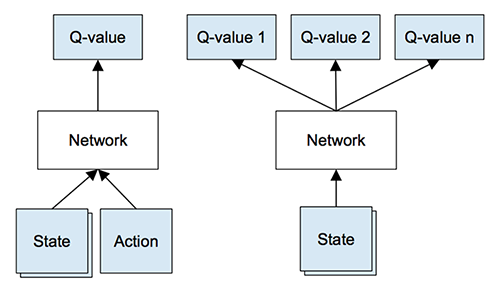
\includegraphics[width=0.8\textwidth]{figs/ch4/architecture-of-deep-q-network}
\caption{Architecture of Deep Q-Network.}
\label{fig:dqn-architecture}
\end{figure}

Although there have been DRL successes with gradient free methods, the vast majority of current work relies on gradients and hence the backpropagation algorithm. The primary motivation is that, when available, gradients provide a strong learning signal. In reality, these gradients are estimated based on approximations, through sampling or otherwise, and as such we have to craft algorithms with useful inductive biases in order for them to be tractable.The other benefit of backpropagation is to view the optimization of the expected return as the optimization of a stochastic function. This function can comprise of several parts' models, policies and value functions, which can be combined in various ways. The individual parts, such as value functions, may not directly optimize the expected return, but can instead embody useful information about the RL domain. For example, using a differentiable model and policy, it is possible to forward propagate and backpropagate through entire rollouts; on the other hand, inaccuracies can accumulate.

If we do all calculations of Deep Neural Network, we will end up with an output, which is actually incorrect. So knowing this we want to update neuron weights and biases so that we get correct results. That?s exactly where backpropagation comes to play. Backpropagation is an algorithm which calculates error gradients with respect to each network variable (neuron weights and biases). Those gradients are later used in optimization algorithms, such as Gradient Descent, which updates them correspondingly. The process of weights and biases update is called Backward Pass.

In order to start calculating error gradients, first, we have to calculate the error (in other words, loss) itself. We will use standard classification loss, cross entropy. However, the loss function could be any differentiable mathematical expression. The standard choice for regression problems would be a Root Mean Square Error (RMSE). The cross entropy loss looks as following:

\begin{equation} \label{eq:reward-func}
L = - \sum_j^M y_j ln p_j
\end{equation}

\vfill
